\documentclass[landscape,a1paper]{tikzposter}

\usepackage{amsmath}
\usepackage{amssymb}

\title{Hyperbolic convolutions}

\begin{document}
\maketitle

\begin{columns}
\column{0.5} \block{Original hyperbolic convolutions for images, DL2019@SkT}{
        \begin{subcolumns}
            \subcolumn{0.5} \innerblock{}{
                \begin{tikzpicture}
                    \node[anchor=south west,inner sep=0pt] at (0,0) {
                        %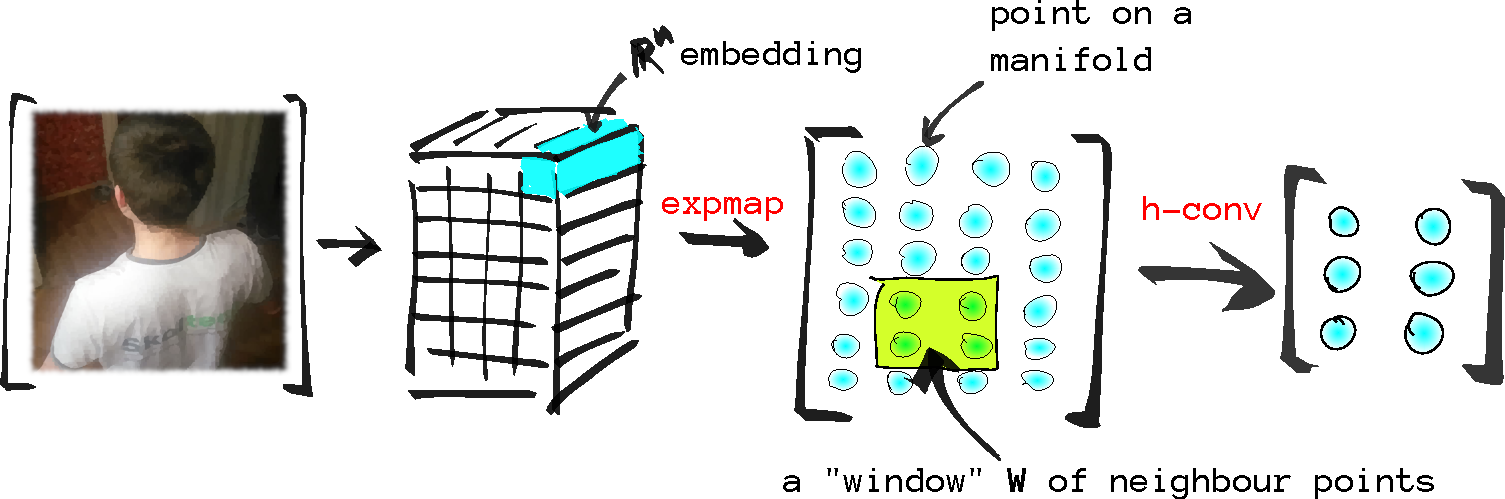
\includegraphics[width=\textwidth]{art/image-convolutions-2019}
                        \input{art/image-convolutions-2019-wide.pdf_tex}
                    };
                    \draw[red,ultra thick,rounded corners] (7.5,5.3) rectangle (9.4,6.2);
                \end{tikzpicture}}
            \subcolumn{0.5} \innerblock{}{
                \begin{align*}
                    Y = \log_0(y),\\
                    Y' = \operatorname{nn.Conv2D}(Y),\\
                    y' = \exp_x(T_{\log_0x}(Y')).
                \end{align*}
            }
    \end{subcolumns}

    Collaboration with Max Kochurov, Rasoul Karimov, Cyrill Mazur, Maria Taktasheva.
}
\column{0.5} \block{Relative directions}{
    \begin{subcolumns}
        \subcolumn{0.5} \innerblock{}{
        \begin{tikzpicture}
            \node[anchor=south west,inner sep=0pt] at (0,0) {
                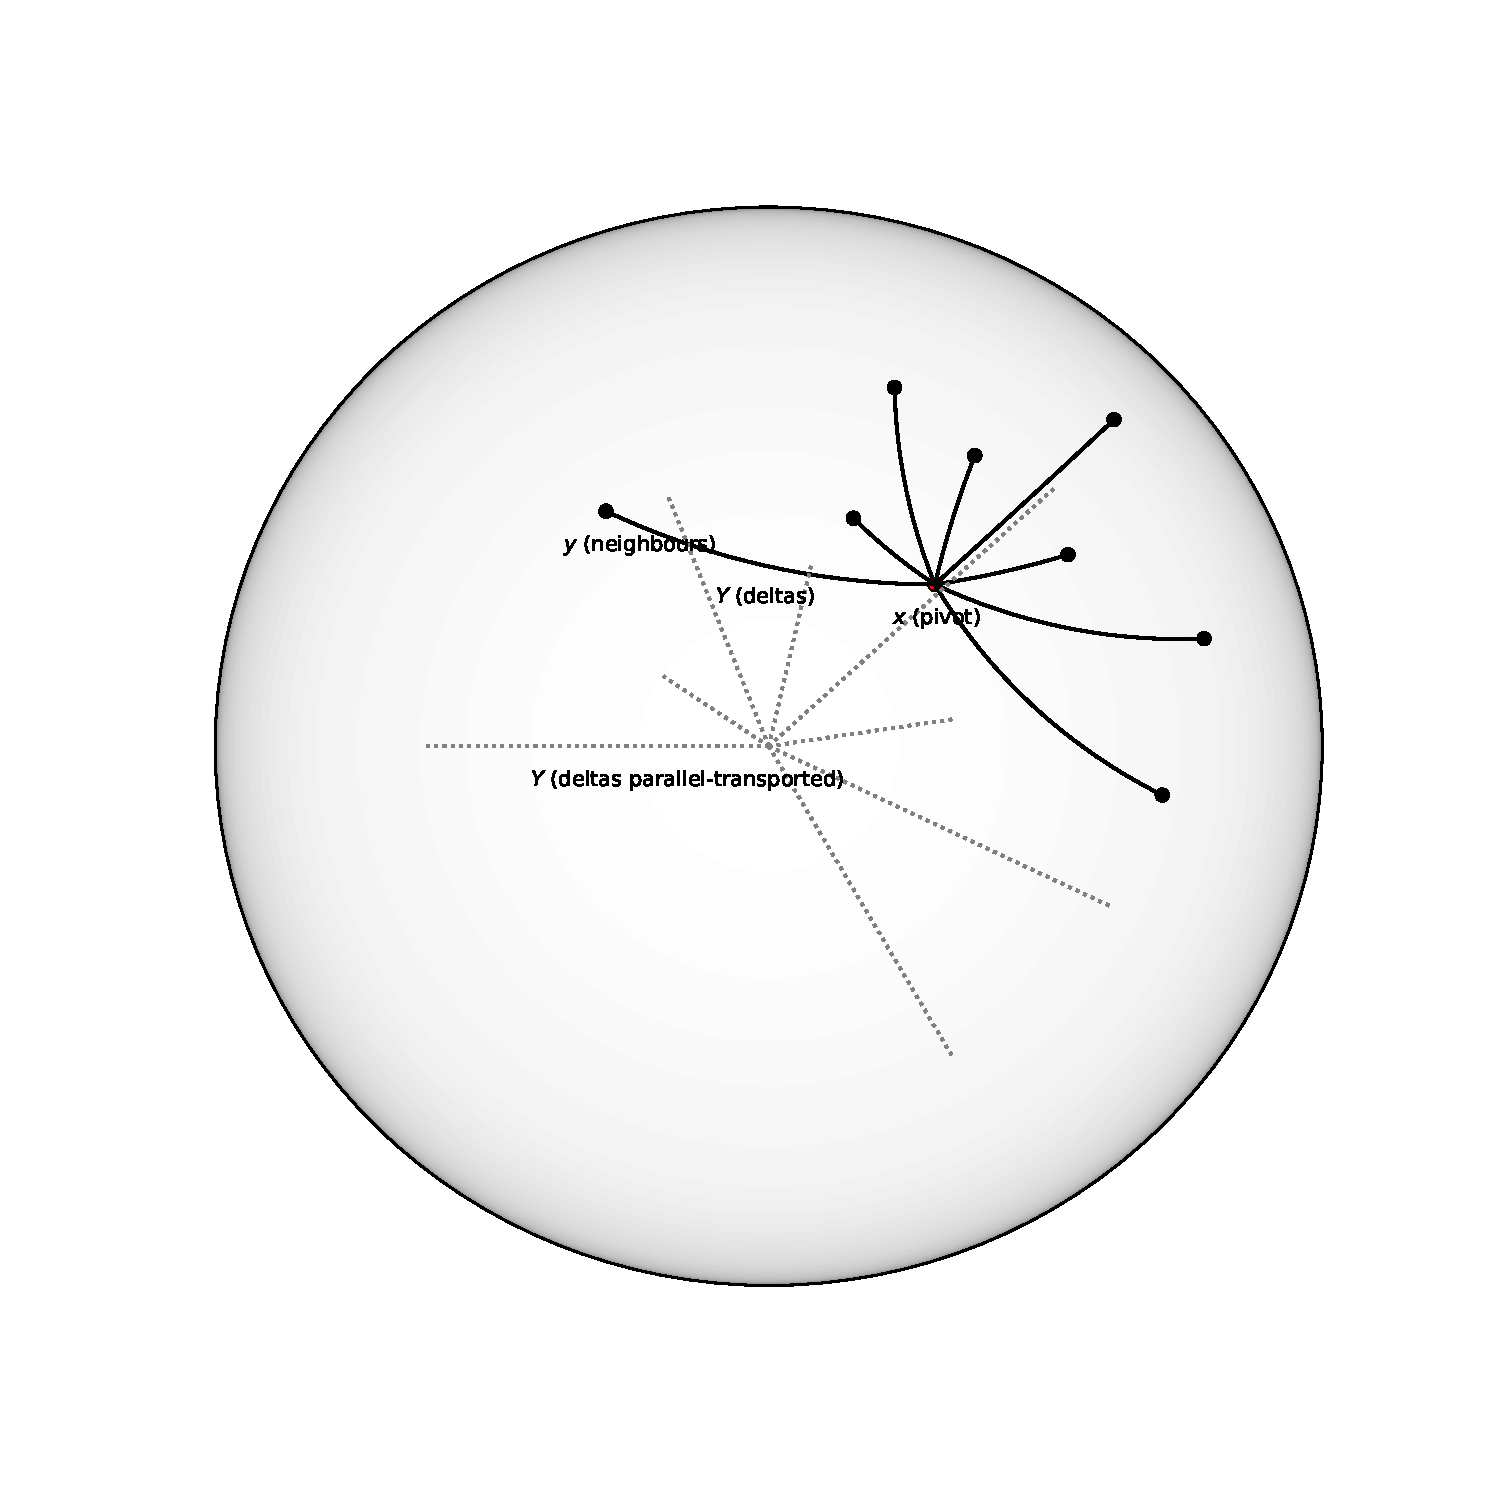
\includegraphics[width=.125\textwidth]{art/neighbours.pdf}
            };
        \end{tikzpicture}
    }
        \subcolumn{0.5} \innerblock{}{
            \begin{align*}
                    x \in \mathcal{W},\\
                    Y = T_{-\log_0x}(\log_x(y))\in T_0M\simeq \mathbb{R}^n,\\
                    Y' = \operatorname{nn.Conv2D}(Y) \in T_xM,\\
                    y' = \exp_x(T_{\log_0x}(Y')). \\
            \end{align*}
        }
    \end{subcolumns}
}
\end{columns}

\block{hyperbolic edgeconv}{
        \begin{tikzpicture}
            \node[anchor=south west,inner sep=0pt] at (0,0) {
                        \def\svgwidth{.7\textwidth}
                        \input{art/hyperbolic-edgeconv.pdf_tex}
            };
        \end{tikzpicture}
}

\end{document}
